\chapter{多类生物标记物定位问题实验评估}\label{sec:multi_classes}
\section{前言}
本章
\section{数据集介绍}
\subsection{多类模拟皮肤病病变数据集}
\begin{figure}[h]
	\centering
	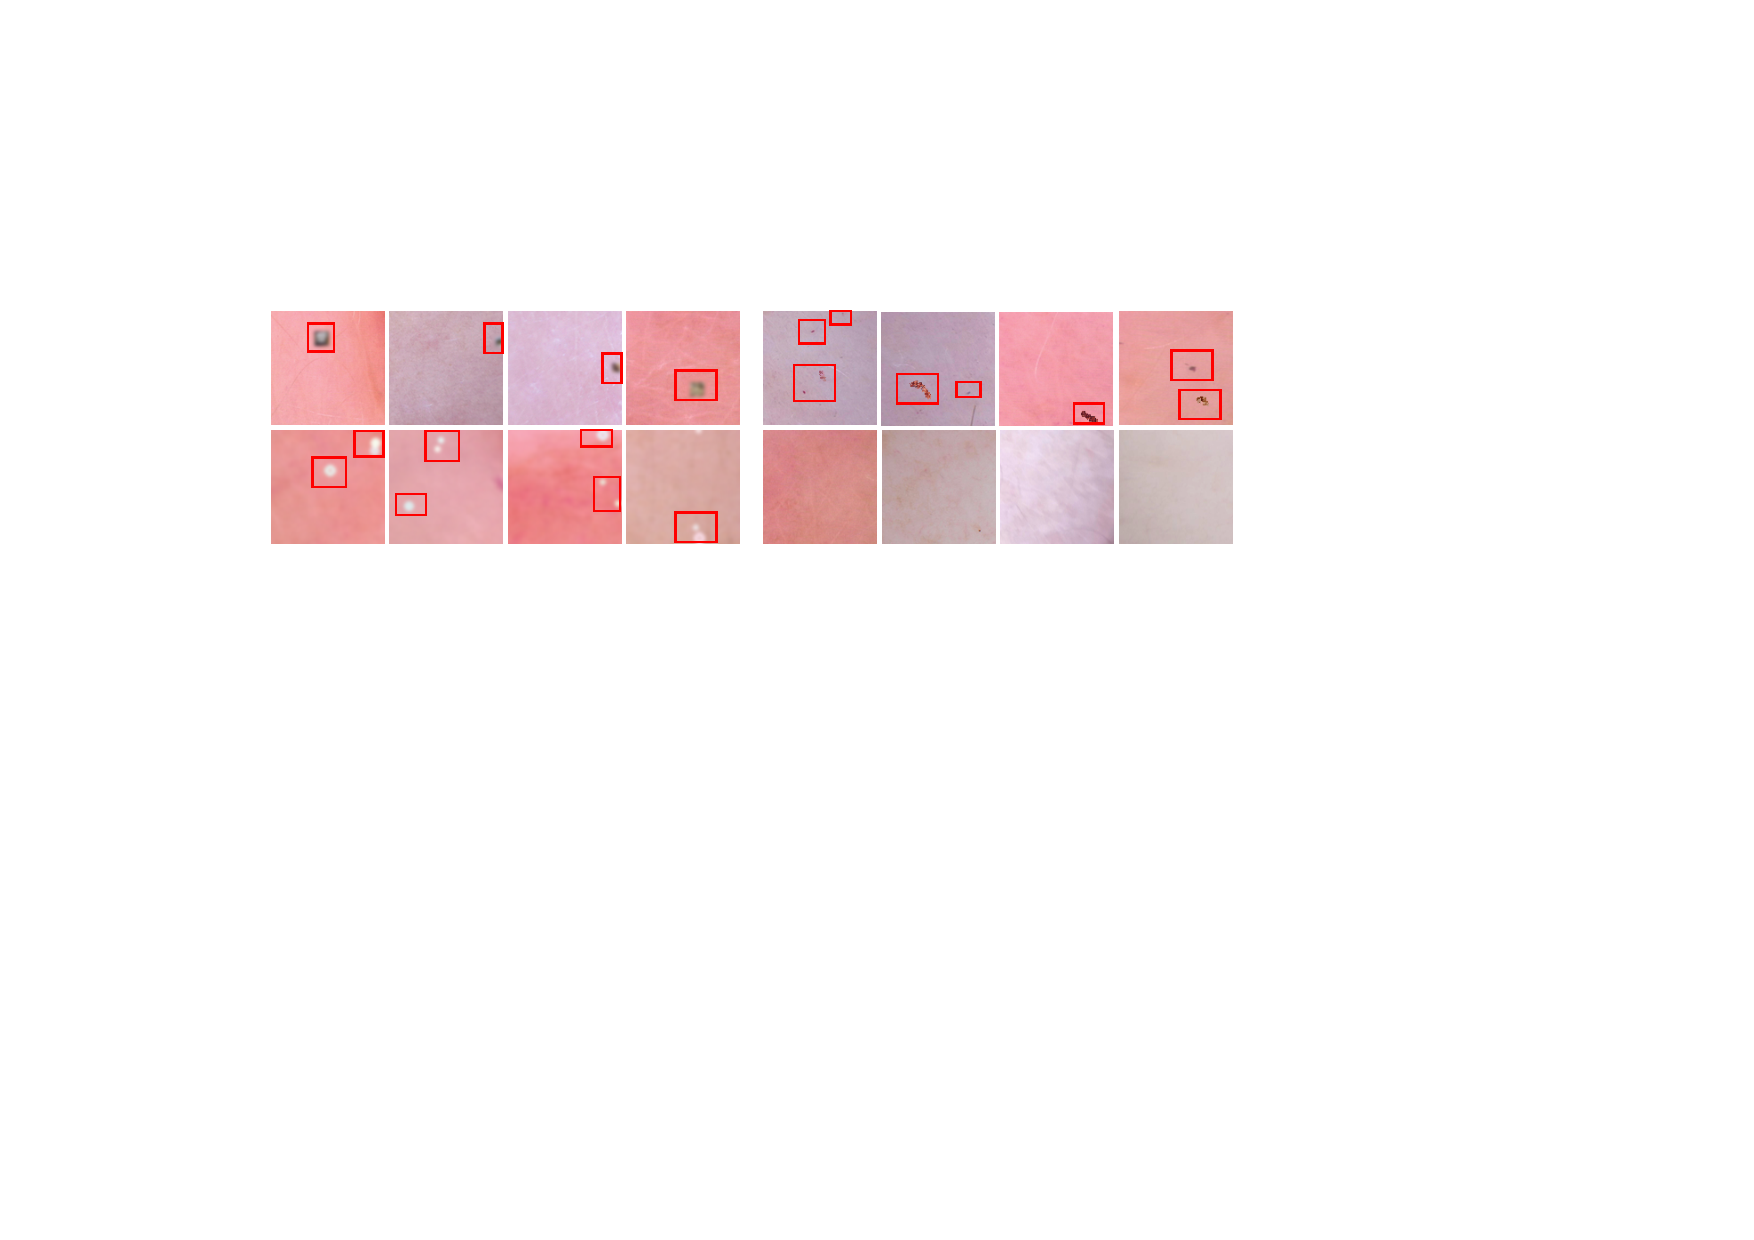
\includegraphics[width=1.0\textwidth]{figure/multi_classes_simulated_skin.pdf}
	\caption{}
	\label{fig:mul_classes_simulated_ds}
\end{figure}

\section{实验设置}
\section{在多类生物标记物定位问题实验评估}
\begin{figure}[h]
	\centering
	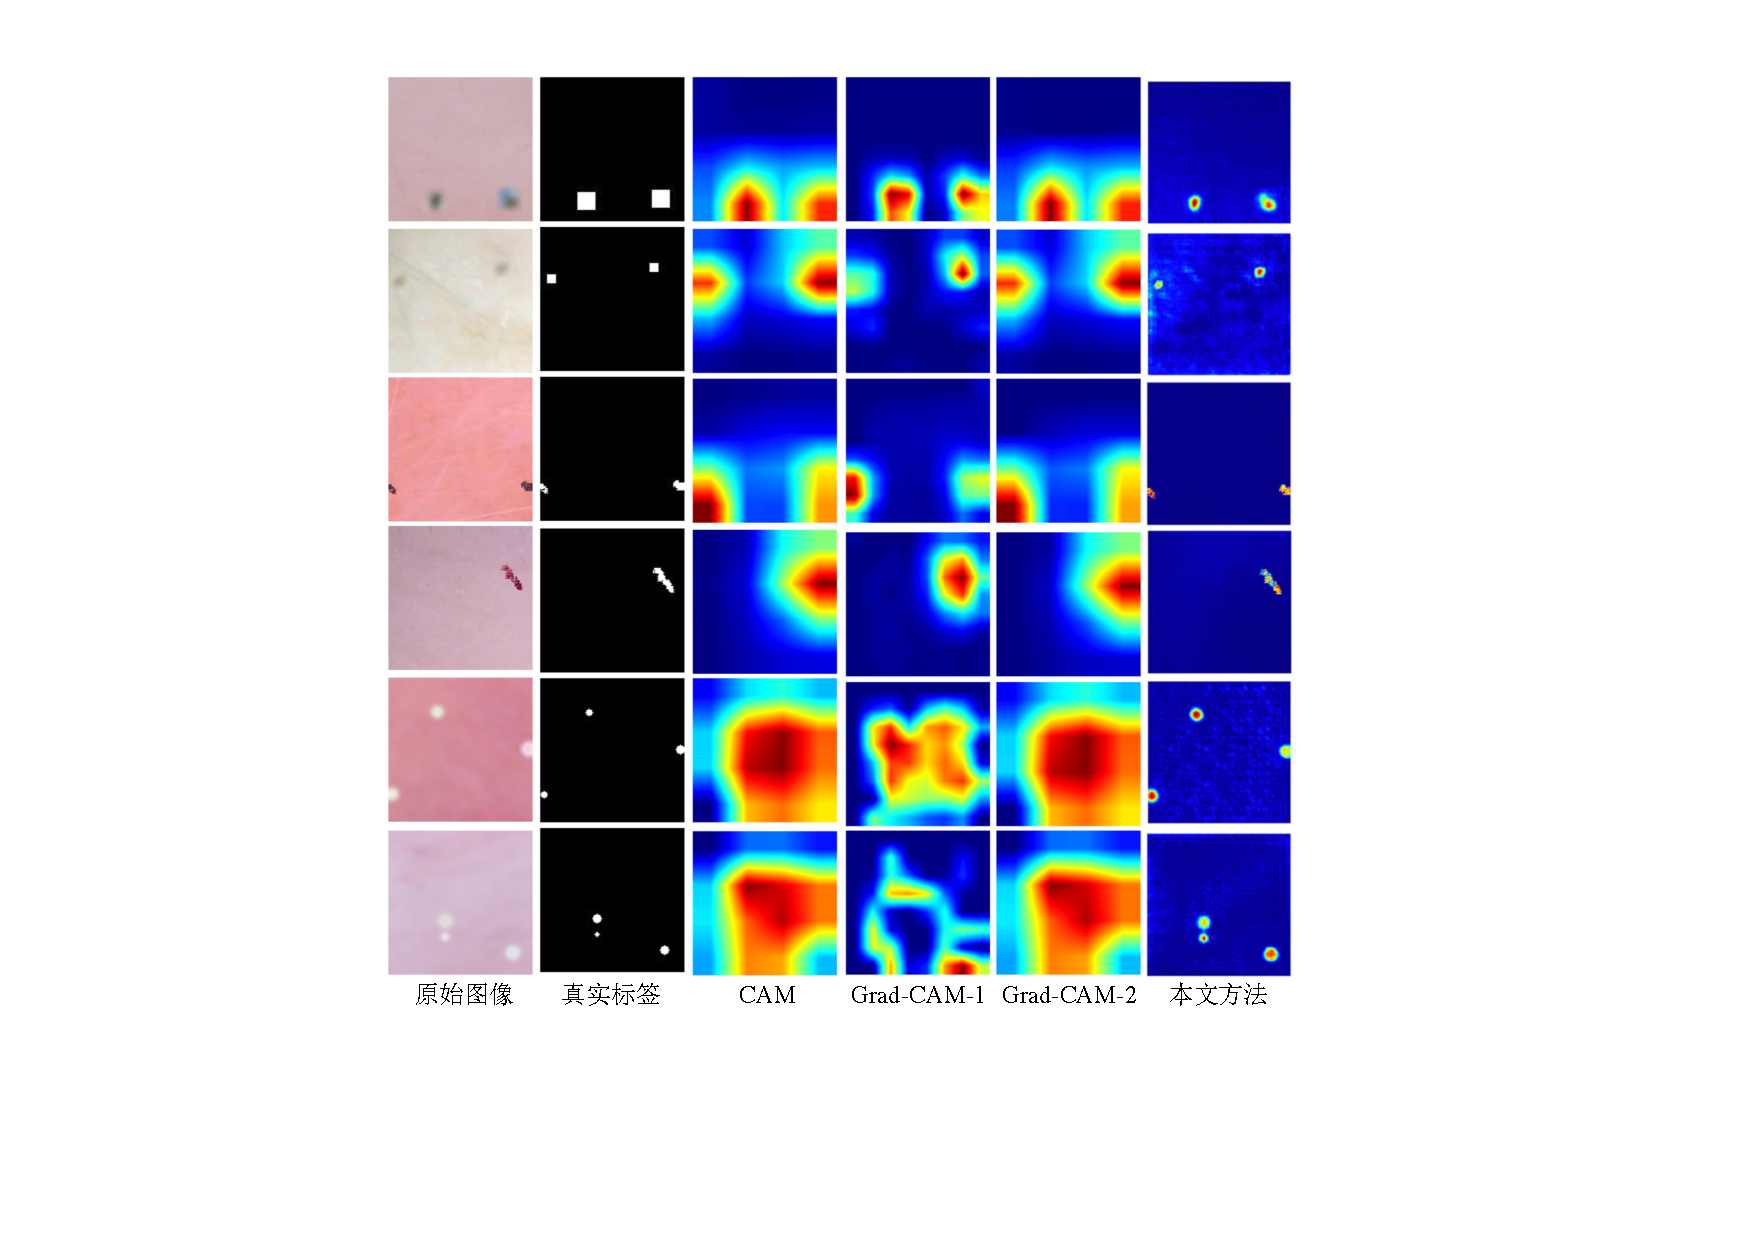
\includegraphics[width=1.0\textwidth]{figure/multi_simulated_skin_res.pdf}
	\caption{}
	\label{fig:multi_simulated_skin_res}
\end{figure}
\section{对于经过编码器-解码器的多类模拟皮肤病病变图像的定量分析}
\section{不同超参数下的实验结果分析}
\section{对判别器模型结构的探究}
\section{本章小结}
